\documentclass[11pt,letterpaper]{article}
\usepackage{amsmath, amssymb}
\usepackage{etoolbox}
\usepackage{graphicx}
\usepackage[round,authoryear]{natbib}
\usepackage{setspace}
\usepackage{booktabs, threeparttable, tabularx, makecell}
\usepackage{indentfirst}
\usepackage{xurl}
\usepackage[colorlinks=true,linkcolor=black,urlcolor=blue,citecolor=black]{hyperref}
\usepackage{float}
\usepackage[affil-it]{authblk}
\usepackage[osf]{mathpazo}
\usepackage[left=2cm,right=2cm,top=1.5cm,bottom=1.5cm]{geometry}
\BeforeBeginEnvironment{tabular}{\footnotesize}
\usepackage{ragged2e}

\makeatletter
\renewcommand{\TPTnoteSettings}{\footnotesize\RaggedRight}
\makeatother

\title{Crop Rotation and the Probability of Covering Costs: A State-by-State Simulation for Eight Corn Belt States}

\author{Victor Funes-Leal}
\author{Lawson Connor}
\author{Eunchun Park}

\affil{Department of Agricultural Economics and Agribusiness, University of Arkansas}

\date{}

\begin{document}

\maketitle

\begin{abstract}
Whether a rotation pays is usually answered with expected returns, but a producer facing thin margins also cares about how often revenue falls short of cost. This paper estimates that breakeven probability, $\Pr(\text{revenue} < \text{cost})$, for continuous corn, a corn-corn-soybean rotation, and strict corn-soybean alternation, separately for each of eight Corn Belt states (Iowa, Illinois, Indiana, Minnesota, Missouri, Ohio, South Dakota, and Wisconsin) and for three soil-productivity zones defined by terciles of the National Commodity Crop Productivity Index (NCCPI). Yields come from a field-level satellite panel and are drawn conditional on each field's six-year crop history; prices, costs, and the price-yield dependence are calibrated state by state. Against 2025 total non-land costs, the probability that a given year's revenue falls below cost is 49 to 69 percent under continuous corn and 35 to 62 percent under strict alternation (medium zone), so the margin is thin enough that breakeven risk, not expected profit, is the relevant yardstick. Strict alternation lowers the annual probability by 7 to 24 percentage points depending on the state, with the largest gains in Ohio and Indiana and the smallest in South Dakota. The six-year cumulative probability of a negative net return falls by 45 points in Ohio and 39 in Indiana, but by only 10 in South Dakota. Zone matters less than state: moving from the high to the low NCCPI tercile raises the annual probability by 2 to 18 points, and the rotation gap is similar in all three zones. Allowing for the negative price-yield correlation changes the annual probability by at most 1.5 points. The rotation advantage is large across states, but its size depends on where the state's mean margin sits relative to zero.
\end{abstract}

\noindent\textbf{Keywords:} Crop rotation; Breakeven probability; Revenue risk; Corn Belt; Simulation

\noindent\textbf{JEL Codes:} Q12, Q14, D81

\clearpage

\section{\label{sec:introduction}Introduction}

Row-crop margins are thin. Budget-based estimates for 2025 put total non-land cost near \$770 per acre for corn and \$435 to \$490 for soybeans across the Corn Belt, close to the revenue those crops earn at benchmark prices. When the mean margin is this near zero, the useful question about a rotation is not whether it raises expected profit by a few dollars, but how much it changes the chance that a season fails to cover cost. That chance, the breakeven probability, is the object this paper estimates.

The agronomic case for rotation is well documented. Corn after corn yields less than corn after soybeans \citep{Bullock1992, Seifert2017}, and diversified rotations reduce yield losses in dry years and compress the lower tail of the yield distribution \citep{Bowles2020, Smith2023}. Yet rotation simplification continues, concentrated on the most productive land \citep{socolar2021}. What has been missing is a statement of the rotation advantage in the units a producer, lender, or insurer reasons in: the probability of failing to cover cost, state by state, with the price and cost environment explicit. We provide the breakeven probability for eight states, each estimated on its own from the same kind of field-level panel and the same simulation, so that differences across states reflect the data and not a change in method.

We simulate six-year revenue and cost paths for each state and each of three NCCPI productivity zones. Yields are drawn nonparametrically from a generator that conditions on the field's full six-year crop history. Prices are lognormal with state means and volatilities calibrated from elevator cash prices; costs are state total non-land budget costs with a same-crop penalty; and the negative price-yield correlation enters through a decomposition that applies it only to the systematic component of yield. We compare continuous corn, a corn-corn-soybean rotation, and strict alternation.

Four findings stand out.

\textbf{First, breakeven risk is high everywhere.} With total non-land cost as the threshold, the annual probability that revenue falls short is 49 to 69 percent under continuous corn and 35 to 62 percent under strict alternation in the medium zone. The chance of at least one shortfall in six years is above 90 percent in every cell, which is why we report annual and cumulative probabilities and not the ``any shortfall'' event.

\textbf{Second, rotation lowers breakeven risk in every state, by very different amounts.} Strict alternation reduces the annual probability by 7 points in South Dakota, by 11 to 14 points in Iowa, Illinois, Minnesota, Missouri, and Wisconsin, and by 23 to 24 points in Indiana and Ohio. The gap tracks the position of the state's mean margin: where continuous corn loses money on average and the rotation recovers a positive margin, replacing corn years moves much of the distribution across the breakeven line.

\textbf{Third, zone matters less than state.} The NCCPI terciles shift the annual probability by 2 to 18 points from the high to the low zone, while the rotation gap is similar across zones within a state.

\textbf{Fourth, price-yield dependence is second order for this outcome.} Switching the negative price-yield correlation on changes the annual probability by at most 1.5 points in any state.

The paper is organized as follows. Section~\ref{sec:framework} defines the breakeven probability and the structural model. Section~\ref{sec:data} describes the panel, zones, prices, and costs. Section~\ref{sec:simulation} describes the simulation. Section~\ref{sec:results} reports results. Section~\ref{sec:discussion} discusses limitations and implications, and Section~\ref{sec:conclusion} concludes.

\section{\label{sec:framework}Framework}

\subsection{Breakeven probability}

Let a field in state $s$ and zone $z$ follow a six-year plan $\pi = (c_1,\dots,c_6)$ with $c_t\in\{C,S\}$ for corn and soybeans, starting from a six-year history $h$. In year $t$ revenue is $R_t = P_t Y_t$, with price $P_t$ for crop $c_t$ and yield $Y_t$ drawn conditional on the six-year window of crops ending in $t$. Cost is $K_t = \bar K_{c_t}^{s}\,\varepsilon_t + \delta_{c_t}\mathbf 1\{c_t = c_{t-1}\}$, where $\bar K^{s}_{c}$ is the state's total non-land cost, $\varepsilon_t$ is a lognormal shock with unit mean, and $\delta_c$ is the extra cost of planting a crop after itself. Year $t$ is a shortfall if $R_t < K_t$. We report, for each state-zone-plan cell:
\begin{itemize}
\item the annual breakeven probability $\bar p = \frac16\sum_t \Pr(R_t<K_t)$;
\item the six-year cumulative probability $\Pr\big(\sum_t (R_t-K_t) < 0\big)$;
\item the mean annual net return $E[R_t-K_t]$.
\end{itemize}
We also record the probability of at least one shortfall in six years, but it is above 90 percent in every cell and is not informative.

\subsection{Mechanism}

Rotation enters through two channels on the path from the plan to $\Pr(R<K)$. The first is yield: the six-year window conditions the yield draw, so the plan changes the mean and dispersion of $Y_t$ in each year. The second is crop composition together with the same-crop cost penalty. Soybeans and corn have different revenue and cost levels, so replacing corn years with soybean years changes the mix of margins even with yields held fixed. The simulation reports the combined effect of the plan; we do not separate the two channels here.

\section{\label{sec:data}Data and calibration}

\subsection{Field panel and productivity zones}

Yields come from a satellite-derived field-level panel of corn and soybean yields for each of the eight states, with a six-year crop history for each field-year. For each state, crop, and zone we estimate a two-way fixed-effects model (field and year) on field-year yields. The generator for each six-year rotation state stores the residuals from that model as an empirical pool and a mean equal to the average field effect of the state's observations plus one common, cell-wide year effect. A draw is the mean plus a resampled residual. Generators are built separately for each state and zone and are never pooled across states.

Zones are terciles of field-level NCCPI, computed within the state from the pooled corn and soybean fields so that a field belongs to one zone for both crops. NCCPI is a soil rating, not a realized yield, so zones are defined by the land and not by the outcome being studied. The terciles are narrow in some states (for Ohio the cut-points are 0.65 and 0.71), and the resulting yield differences between zones are correspondingly modest.

\subsection{Prices, costs, and dependence}

\begin{table}[H]
\centering
\caption{State inputs. Price is the 2025 budget benchmark (\$4.20 corn, \$10.25 soybeans, Illinois) scaled by each state's elevator basis; $\sigma$ is the standard deviation of elevator-demeaned log harvest-season prices; cost is total non-land cost per acre; BE yield is cost divided by mean price (bu/ac).}
\label{tab:inputs}
\begin{threeparttable}
\begin{tabular}{lcccccccc}
\toprule
& \multicolumn{4}{c}{Corn} & \multicolumn{4}{c}{Soybeans}\\
\cmidrule(lr){2-5}\cmidrule(lr){6-9}
State & Price & $\sigma$ & Cost & BE yield & Price & $\sigma$ & Cost & BE yield\\
\midrule
IA & 4.17 & 0.242 & 771 & 185 & 9.93 & 0.185 & 453 & 45.6 \\
IL & 4.20 & 0.227 & 768 & 183 & 10.25 & 0.173 & 490 & 47.8 \\
IN & 4.29 & 0.215 & 836 & 195 & 10.24 & 0.170 & 455 & 44.4 \\
MN & 4.03 & 0.259 & 771 & 191 & 9.89 & 0.193 & 457 & 46.2 \\
MO & 4.17 & 0.242 & 744 & 178 & 10.12 & 0.184 & 459 & 45.4 \\
OH & 4.25 & 0.213 & 780 & 184 & 10.15 & 0.169 & 436 & 43.0 \\
SD & 3.94 & 0.268 & 748 & 190 & 9.72 & 0.200 & 456 & 46.9 \\
WI & 4.03 & 0.235 & 769 & 191 & 9.78 & 0.180 & 460 & 47.0 \\
\bottomrule
\end{tabular}

\begin{tablenotes}
\item Total non-land cost is published for Illinois (farmdoc) and computed for Ohio as total cost minus land (OSU). For the other six states only direct cost is available, and we add the mean of the Illinois and Ohio non-direct costs (\$296 per acre for corn, \$243 for soybeans); results for these six states inherit that assumption.
\end{tablenotes}
\end{threeparttable}
\end{table}

\textbf{Prices.} Prices are lognormal. The mean is the common 2025 budget benchmark times a state basis, estimated as the state coefficient in a regression of log harvest-season elevator cash price on state and year effects, relative to Illinois. Using the budget benchmark puts revenue and cost in the same year. The volatility is the standard deviation of elevator-demeaned log prices within each state and crop.

\textbf{Costs.} Costs are lognormal around the state's total non-land cost with a log standard deviation of 0.10. Planting a crop after itself adds \$15 per acre for corn and \$5 for soybeans, the Illinois budget differences. Land is excluded so that the threshold does not depend on rent differences across states.

\textbf{Price-yield dependence.} We use the decomposed method: a normal aggregate yield shock that carries 40 percent of yield variance and is correlated with the log-price shock, plus an independent idiosyncratic shock. The correlation is the state median of county-level price-yield correlations.

\section{\label{sec:simulation}Simulation}

For each state, zone, and plan we simulate 50,000 six-year paths. Each plan is run from a history equal to the plan itself, so it starts in steady state. The three plans are continuous corn (CCCCCC), corn-corn-soybean (CCSCCS), and strict alternation (CSCSCS). Random draws are shared across plans within a state-zone cell (common random numbers) and cells use independent seeds, so differences across plans within a cell are not Monte Carlo noise. Every cell is run with and without price-yield dependence.

\section{\label{sec:results}Results}

\subsection{Breakeven probabilities by state and rotation}

\begin{table}[H]
\centering
\caption{Breakeven probabilities, medium NCCPI zone (percent). Annual: $\Pr(R_t<K_t)$ in a given year. Cumulative: $\Pr(\sum_t (R_t-K_t)<0)$ over six years. Gap: strict alternation minus continuous corn, annual, in percentage points.}
\label{tab:main}
\begin{tabular}{lcccccc}
\toprule
& \multicolumn{3}{c}{Annual} & \multicolumn{2}{c}{Six-year cumulative} & \\
\cmidrule(lr){2-4}\cmidrule(lr){5-6}
State & CCCCCC & CCSCCS & CSCSCS & CCCCCC & CSCSCS & Gap (pp)\\
\midrule
IA & 50.0 & 40.4 & 38.3 & 42.2 & 25.9 & -11.7 \\
IL & 48.6 & 39.6 & 37.9 & 40.0 & 24.1 & -10.7 \\
IN & 64.1 & 48.7 & 41.6 & 76.6 & 37.6 & -22.5 \\
MN & 58.1 & 48.5 & 47.0 & 61.7 & 41.5 & -11.1 \\
MO & 60.5 & 51.8 & 49.3 & 67.4 & 50.7 & -11.2 \\
OH & 58.7 & 40.5 & 34.5 & 64.8 & 20.0 & -24.2 \\
SD & 69.2 & 64.1 & 62.1 & 84.2 & 74.3 & -7.1 \\
WI & 68.3 & 56.5 & 54.6 & 83.1 & 61.6 & -13.7 \\
\bottomrule
\end{tabular}

\end{table}

Table~\ref{tab:main} and Figure~\ref{fig:annual} report the annual probabilities. Under continuous corn the probability that a year's revenue falls below total non-land cost ranges from 48.6 percent in Illinois to 69.2 percent in South Dakota. Under strict alternation it ranges from 34.5 percent in Ohio to 62.1 percent in South Dakota. The corn-corn-soybean rotation sits between the two in every state. Illinois and Iowa have the lowest probabilities under continuous corn, and South Dakota and Wisconsin the highest. The breakeven corn yield is similar across states (178 to 195 bu/ac at mean price, Table~\ref{tab:inputs}), so the ranking reflects how far each state's simulated revenue sits from its cost, together with price level and volatility.

\begin{figure}[H]
\centering
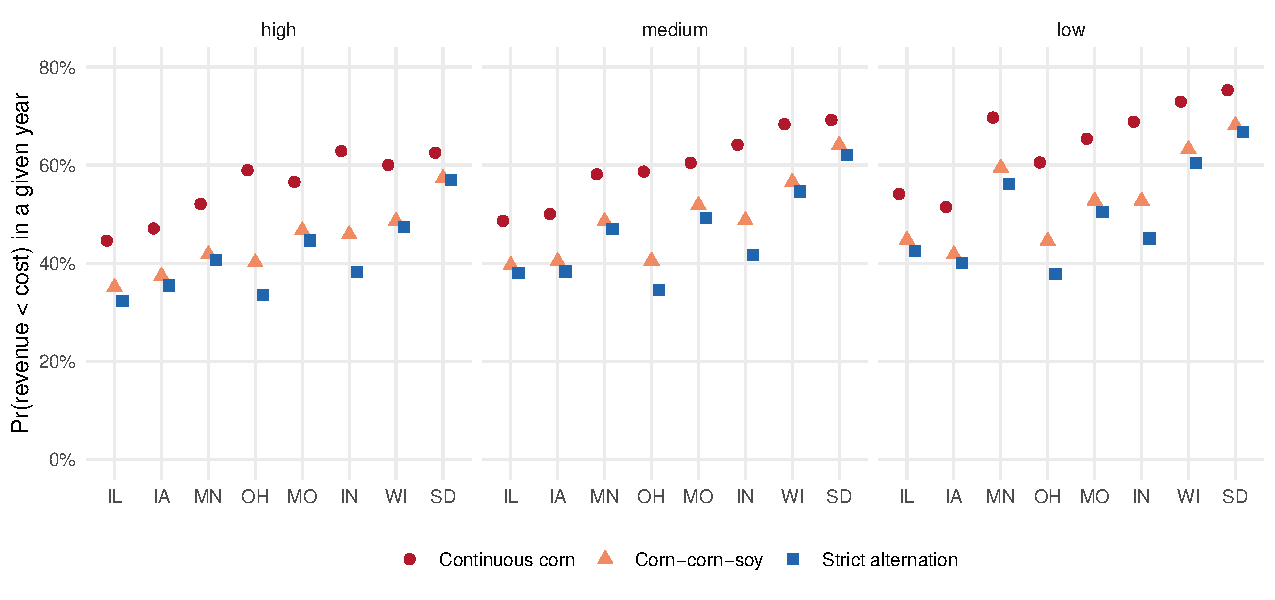
\includegraphics[width=\textwidth]{figs/be_p_loss_year.pdf}
\caption{Annual probability that revenue falls below total non-land cost, by state, rotation, and NCCPI zone. States are ordered by the continuous-corn probability in the medium zone.}
\label{fig:annual}
\end{figure}

The six-year cumulative probability tells the same story with larger gaps. The probability that cumulative net return over six years is negative is 40 to 84 percent under continuous corn and 20 to 74 percent under strict alternation (Figure~\ref{fig:cum}). The drop is 39 points in Indiana, 45 points in Ohio, and 10 points in South Dakota.

\begin{figure}[H]
\centering
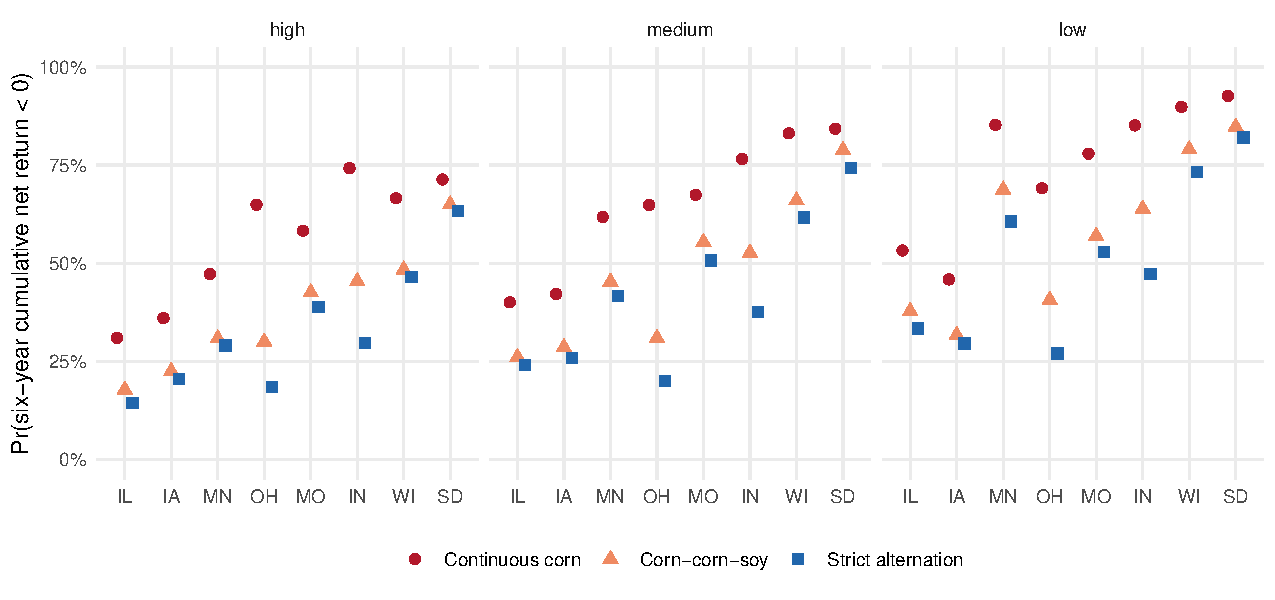
\includegraphics[width=\textwidth]{figs/be_p_loss_cum.pdf}
\caption{Probability that the six-year cumulative net return is negative, by state, rotation, and NCCPI zone.}
\label{fig:cum}
\end{figure}

\subsection{The rotation gap}

\begin{figure}[H]
\centering
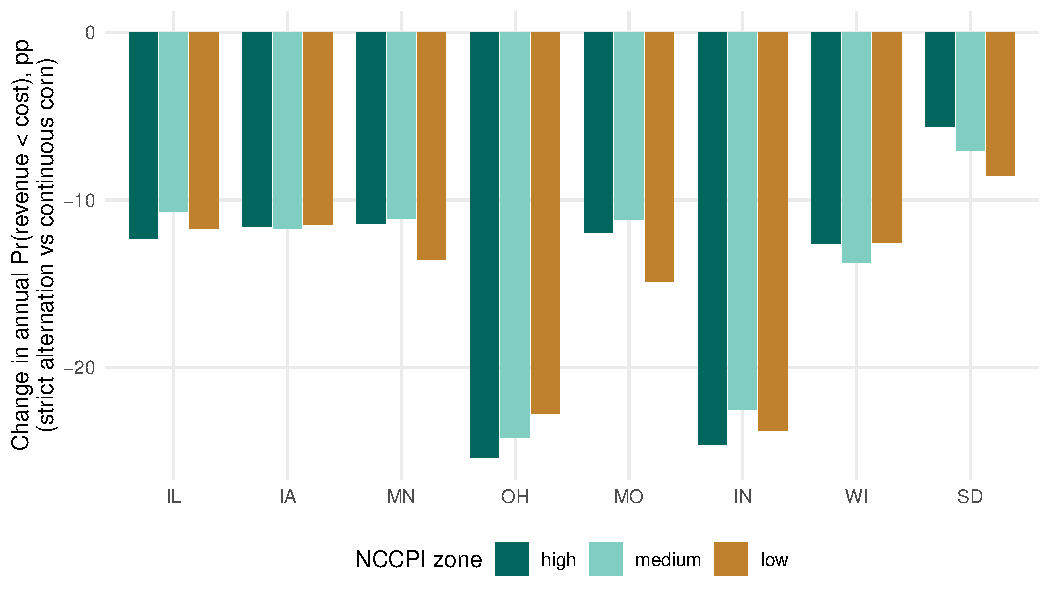
\includegraphics[width=0.75\textwidth]{figs/be_rotation_gap.pdf}
\caption{Change in the annual breakeven probability from continuous corn to strict alternation, by state and NCCPI zone (percentage points).}
\label{fig:gap}
\end{figure}

Figure~\ref{fig:gap} shows the reduction from continuous corn to strict alternation. It is 5.6 to 8.6 points in South Dakota, 10.7 to 14.9 points in Iowa, Illinois, Minnesota, Missouri, and Wisconsin, and 22.5 to 25.4 points in Indiana and Ohio. The reduction is similar across zones within a state, so the ranking of states reflects state-level margins and not soil quality. The mean margins in the medium zone explain the pattern. Continuous corn earns a positive mean margin in Iowa and Illinois (about \$20 to \$24 per acre per year), a mildly negative one in Minnesota, Missouri, and Ohio (\$22 to \$33), and a strongly negative one in Indiana, Wisconsin, and South Dakota (\$55 to \$80). Strict alternation lifts the mean margin to positive values in Indiana (\$22), Ohio (\$52), and Minnesota (\$17), so in Indiana and Ohio the rotation moves most of the distribution across the breakeven line. In South Dakota and Wisconsin both plans lose on average, and the rotation narrows the shortfall without removing it.

\subsection{Productivity zones}

\begin{table}[H]
\centering
\caption{Annual breakeven probability by NCCPI zone (percent).}
\label{tab:zone}
\begin{tabular}{lcccccc}
\toprule
& \multicolumn{3}{c}{Continuous corn} & \multicolumn{3}{c}{Strict alternation}\\
\cmidrule(lr){2-4}\cmidrule(lr){5-7}
State & High & Medium & Low & High & Medium & Low\\
\midrule
IA & 47.1 & 50.0 & 51.4 & 35.5 & 38.3 & 40.0 \\
IL & 44.6 & 48.6 & 54.1 & 32.3 & 37.9 & 42.4 \\
IN & 62.8 & 64.1 & 68.8 & 38.3 & 41.6 & 45.1 \\
MN & 52.1 & 58.1 & 69.7 & 40.6 & 47.0 & 56.1 \\
MO & 56.6 & 60.5 & 65.4 & 44.6 & 49.3 & 50.5 \\
OH & 58.9 & 58.7 & 60.5 & 33.5 & 34.5 & 37.8 \\
SD & 62.5 & 69.2 & 75.2 & 56.9 & 62.1 & 66.7 \\
WI & 60.0 & 68.3 & 72.9 & 47.4 & 54.6 & 60.4 \\
\bottomrule
\end{tabular}

\end{table}

Table~\ref{tab:zone} shows that moving from the high to the low NCCPI tercile raises the continuous-corn annual probability by 1.6 points in Ohio, 4.3 in Iowa, 6.0 in Indiana, 8.8 in Missouri, 9.5 in Illinois, 12.7 in South Dakota, 12.9 in Wisconsin, and 17.6 in Minnesota. Zone effects are real but modest in several states. Because the terciles cut a narrow band of the soil index in some states, NCCPI is a weak sorter of breakeven risk relative to state.

\subsection{Price-yield dependence}

Turning off the price-yield correlation changes the annual probability by at most 1.5 points in any state and plan (medium zone). For an annual comparison of revenue with cost, the dependence changes the dispersion of revenue slightly but not its mean, and the location of the mean relative to cost dominates. The dependence is therefore not a source of the rotation advantage here.

\section{\label{sec:discussion}Discussion}

\textbf{What the results say.} Where the mean margin is near zero, a rotation that adds a few dollars per acre of expected margin shifts the breakeven probability by tens of points. The gap is therefore not proportional to the expected-return benefit. It is largest where continuous corn loses on average and the rotation brings the mean margin to or above zero (Indiana, Ohio), and smallest where both plans lose on average (South Dakota).

\textbf{Limitations.} First, costs for six states rest on an assumed non-direct cost; the level of every probability in those states depends on it, and the ranking of states is sensitive to it. Replacing the assumed add-on with state budget values is the most important refinement. Second, benchmark prices follow the 2025 budgets, so results describe a 2025 price and cost environment and not the period over which yields are estimated; a sweep over the mean price is the natural extension, since the breakeven probability is a function of the price level. Third, the plan comparison combines the yield effect of rotation with the change in crop mix and the same-crop cost penalty; we do not decompose them. Fourth, NCCPI zones sort breakeven risk weakly in several states, so zone-level conclusions should not be over-read. Fifth, land cost is excluded, so these probabilities describe covering the cost of operating the crop and not of covering rent. Sixth, the generators resample field-level residuals, so each state's within-state yield correlation across fields is not modeled; the results describe an individual field.

\textbf{Relation to the delinquency analysis.} An earlier version of this project studied how unpaid operating loans roll forward and compound in Illinois. That analysis is retained separately. The breakeven probability studied here is the one-year building block of that process and does not require credit terms, which makes it comparable across states.

\section{\label{sec:conclusion}Conclusion}

Across eight Corn Belt states estimated separately, a year of continuous corn fails to cover total non-land cost about half the time or more, and replacing it with strict corn-soybean alternation lowers that probability in every state and every productivity zone, by 6 to 25 percentage points. The effect is largest where the continuous-corn margin is most negative but the rotation restores a positive margin, and smallest in South Dakota. Soil productivity and price-yield dependence matter much less than the state-level margin. The practical implication is that the rotation case rests on where margins sit relative to cost, and that a producer or lender comparing rotations should look at the probability of falling short and not only at expected return. State-specific budget costs, a price sweep, and a separation of the yield and composition channels are the next steps.

\clearpage
\bibliographystyle{apalike}
\bibliography{references}

\end{document}
